% https://topanswers.xyz/tex?q=1302#a1542
\documentclass{beamer}

\beamertemplatenavigationsymbolsempty
\setbeamersize{text margin left=10mm,text margin right=5mm} 
\setbeamertemplate{frametitle}[default][center]
\usepackage{tikz}
\usetikzlibrary{patterns,decorations.pathreplacing}

\begin{document}
\begin{frame}{}
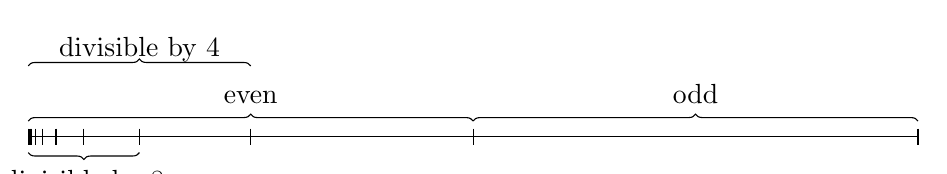
\begin{tikzpicture}
\draw[-] (0,0) -- (11.3,0) ; %edit here for the axis
\foreach \x in  {11.3, 5.65, 2.825, 1.4125, 0.70625, 0.353125, 0.1765625, 0.08828125, 0.044140625, 0.0220703125,0} % edit here for the vertical lines
\draw[shift={(\x,0)},color=black] (0pt,3pt) -- (0pt,-3pt);
\draw [
    decoration={
        brace,
        raise=0.2cm
    },
    decorate
] (5.65,0) -- node[above=2ex] {odd} (11.3,0);
\draw [
    decoration={
        brace,
        raise=0.2cm
    },
    decorate
] (0,0) -- node[above=2ex] {even} (5.65,0);

\draw [
    decoration={
        brace,
        raise=0.9cm
    },
    decorate
] (0,0) -- node[above=5.5ex] {divisible by $4$} (2.825,0);
\draw [
    overlay,
    decoration={
        brace,
        mirror,
        raise=0.2cm
    },
    decorate
] (0,0) -- node[below=2ex] {divisible by $8$} (1.4125,0);
\draw [overlay,
    decoration={
        brace,
        mirror,
        raise=0.9cm
    },
    decorate
] (0,0) -- node[below=5.5ex] {div.\@ by $16$} (0.70625,0);

\end{tikzpicture}
\end{frame}
\end{document}